\documentclass[11pt,a4paper]{article}
\usepackage[margin=24mm]{geometry}
\usepackage{tikz}
\usetikzlibrary{arrows.meta,positioning}
\usepackage[hidelinks]{hyperref}
\title{Compiler repeated work: profile, reduce, verify}
\date{Created-at: 2026-09-07 12:48 +02:00}
\begin{document}
\maketitle
\paragraph{Scope and ETA.} Investigate cold source compilation, AST copying,
reference resolution and repeated traversals. Approximately 45 minutes:
10 minutes instrumentation, 10 minutes profiles and baseline, 15 minutes
implementation and correctness, 10 minutes repeat measurements and report.
Generation, parsing, lowering, hashing, prepared compilation and destruction
remain distinct measurement scopes. Do not remove validation or change hashes.
\paragraph{Authority and checkout.} User requested optimization and investigation
of repeated calls. Core fetched successfully at 12:42--12:45 using the existing
origin with an SSH HostName override for 192.168.1.228; normal DNS failed.
Base is freshly fetched origin/main f305ade; branch perf/compiler-repeated-work
reuses the existing checkout. Former branch 2d43e82 has three unmerged diagnostic
commits and is preserved. Untracked distributed-verification artifacts are preserved.
\paragraph{Discovery.} Extend the existing interning Criterion benchmark and
ModuleStore integration tests. ir\_bench explicitly excludes parsing/lowering;
ir\_depth\_probe measures depth failure, not compilation. Historical CPU optimization
and CBOR reports contain no equivalent compiler profile. Ecosystem reader confirms
Core owns compilation and is consumed by Graph, Transformation and Python.
\paragraph{Affected files.} This four-format plan;
\texttt{hymeko\_core/benches/interning\_bench.rs};
\texttt{hymeko\_core/tests/minimal\_tests/test\_module\_store/test\_module\_store.rs};
candidate production files
\texttt{hymeko\_core/src/module\_store/module\_store.rs},
\texttt{hymeko\_core/src/ir/lower.rs},
\texttt{hymeko\_core/src/ir/canonical\_hash.rs},
\texttt{hymeko\_core/src/resolution/resolve.rs};
\texttt{reports/2026-09-07-compiler-repeated-work.md} and associated numerical,
profile and figure evidence under \texttt{reports/compiler-repeated-work/}.
\paragraph{Core protection.} User approved at the 2026-09-07 continuation:
\texttt{APPROVED-CORE-EDIT: compiler-repeated-work}.
Instrumentation is allowlisted; candidate production files are lockdown-full.
Apply the prepared root-AST/dependency-list borrow patch first, keeping imports,
hashing and validation unchanged. Compare exact IR output (only timestamp normalized),
then cold compilation and cached lookup. Preserve before/after binaries and PDBs.
The user's runtime question also requires quoting the existing prepared Dijkstra
results separately: compiler speedups are not traversal-kernel speedups.
\paragraph{Interfaces and invariants.} Retain public signatures, cache behavior,
resolution ambiguity/error order, import namespace order, IR contents and hash bytes.
The legacy Merkle pass writes serialized decl\_hash and is not redundant merely
because another hash pass exists. No dependency changes. If borrowing ASTs requires
an API change, keep the public owned-slice API and share the underlying lowering.
\paragraph{Measurement and tests.} Criterion release, minimum five post-warmup
iterations; save raw samples, median/IQR/worst. Windows samply CPU profile with
symbols before selecting a hot spot. Read existing Graph campaign artifacts first.
One large production-scale smoke precedes repeated large runs. Record process peak
working set, host and toolchain. Differential whole-IR checks normalize only metadata
timestamps and pin both canonical and declaration hashes; import, constants, aliases,
empty inputs and failure cases. Run relevant and workspace tests, fmt, clippy,
symbols, duplication and preflight. Benchmark same machine and build settings.
\paragraph{Budgets and risk.} Maximum 16 GiB RSS, 180 seconds per measured process;
the existing 50,000-node source provides a quick discriminating workload, followed by
the graph map512 source (30,032,345 bytes) if available through the existing harness.
Target measurable reductions without greater than 10 percent time or memory regression.
No claimed speedup without profile attribution. Nested imports and ambiguous reference
paths can invalidate naive early return or memoization; tests must preserve them.
Cloning may contribute memory rather than dominant CPU cost. Retaining cache entries
may exchange speed for unbounded memory, so do not extend cache lifetime speculatively.
\paragraph{Rollback.} Revert only this task's named changes. Preserve user files,
previous branches, benchmark data and public hash/wire contracts.
\paragraph{Continuation, 2026-09-07 13:36.} Under the same approved slug, strengthen
source-to-IR compilation by reusing the canonical path table between validation and
hashing. A crate-private CanonicalPaths view borrows the IR and owns just its derived
paths; the IR cannot change during its lifetime. Public standalone APIs delegate to
the same methods. Validation borrows index paths rather than cloning them, preserving
the original index iteration and first-error order. Existing DerivedPathIndex also
sorts a lookup table and is therefore inappropriate for this transient compile phase.
Extend existing ModuleStore tests to compare compiled and standalone hashes, and to
exercise namespace corruption. Frozen hashes and full serialized-IR goldens remain
unchanged. Compare the already optimized root-borrow binary against this one change
first; only then consider repeated leaf hashing. Expected additional work: 20 minutes
including two bounded measurement pairs, tests, coverage and report. Retain the
50k baseline and add a larger existing frontend-generator scale if the smoke fits
the declared 16 GiB / 180-second process budget. No second benchmark framework.
\paragraph{Continuation, 2026-09-07 13:59.} Profile-guided compact Pruefer state:
the resolved final profile puts 19.1 percent of compile-stack samples in
prufer\_from\_forest. Replace its HashMap of dense declaration IDs with a dense
vector and per-vertex adjacency lists with degree plus neighbor XOR. For degree one,
the XOR equals the sole remaining neighbor, and removing an edge XORs out its
endpoint. Preserve the existing heap key/order, labels, token sequence, super-root
handling and hash domains. No public API or dependency change; same Core approval.
Extend hymeko\_core/tests/unified\_ir/verification/frozen\_hash.rs before production edits with deterministic
chains, stars, balanced trees, multiple roots, empty and single-node forests,
interleaved anonymous declarations and nondefault hash configuration. Freeze an
aggregate digest against the current shared-path version before the rewrite.
Reuse its archived binary as the immediate baseline. Measure cold compile and
standalone canonical hashing at 50k, then cold compile at the already validated
500k scale in ABBA order; caps remain 180 seconds and 16 GiB per process. Capture
a resolved after-profile, execute workspace tests, clippy and coverage, and append
to the same report. ETA about 15 minutes: targeted parity/build 3, bounded A/B 6,
profile plus checks/report 6. Roll back only this continuation if parity fails or
investigation finds a regression. Existing root-borrow and shared-path edits remain.
\paragraph{Continuation, 2026-09-07 20:06.} Remove duplicate annotation-value
resolution in resolve\_signed\_refs under the existing
\texttt{APPROVED-CORE-EDIT: compiler-repeated-work}. Fresh fetch confirms
HEAD equals origin/main f305ade; preserve all earlier dirty changes. The exact
current profile attributes 610 of 8070 compile samples to this function.
Resolve the annotation once and clone its resolved value into the existing weights
field; both owned wire fields must remain. Preserve list depth, absent versus empty,
floating-point bits, symbol insertion order and first error. Extend existing
test\_ref\_values.rs with mixed-value and error controls before editing production;
extend the normalized-IR corpus for the real-parser path. Extend the existing
Criterion generator with an explicit mixed-reference payload, retaining the numeric
fixture and distinct benchmark identities. Archive matched binaries; compare lowering
and cold compile in ABBA order, ten samples after warmup, with raw samples, IQR,
worst and process peak. Existing 50k and 500k numeric fixture bounds apply; mixed
50k smoke must precede repeated runs. Each process capped at 180 seconds / 16 GiB.
ETA approximately 20 minutes: tests and baseline 5, implementation and measured
pairs 7, workspace gates and report/audit 8. No API or dependency changes.
Bounded audit covers ModuleStore, intern/constant/reference resolution and lowering;
record proven repeated work separately from unmeasured candidates and necessary
semantic passes. Other candidates are not automatically bundled into this patch.
\begin{center}% 2026-10-11: profile merged Core with the existing Criterion workloads;
% keep CPU sampling separate from repeated latency and peak-working-set results.
% Second optimization: borrow Index paths, retain all hierarchy checks and report ordering.
% Third optimization: share immutable Interner data; detach on writes and retain only live strings.
% Shared IR: owned construction -> shared published tables -> detach on first mutation.
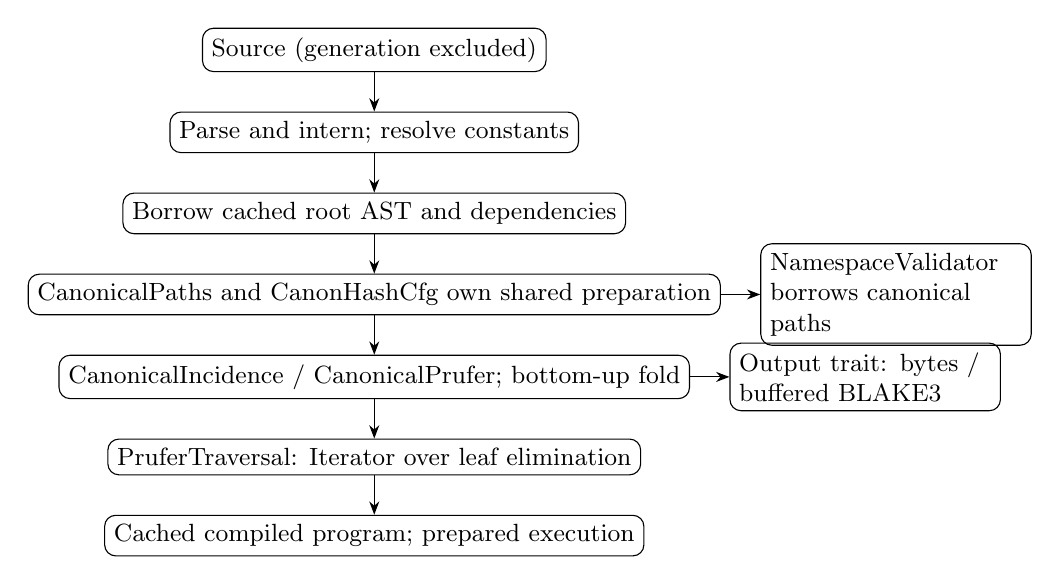
\begin{tikzpicture}[node distance=5mm, every node/.style={draw,rounded corners,font=\small},>=Stealth]
\node (s) {Source (generation excluded)};
\node (p) [below=of s] {Parse and intern; resolve constants};
\node (c) [below=of p] {Borrow cached root AST and dependencies};
\node (i) [below=of c] {CanonicalPaths and CanonHashCfg own shared preparation};
\node (h) [below=of i] {CanonicalIncidence / CanonicalPrufer; bottom-up fold};
\node (t) [below=of h] {PruferTraversal: Iterator over leaf elimination};
\node (o) [right=of h,text width=32mm] {Output trait: bytes / buffered BLAKE3};
\node (v) [right=of i,text width=32mm] {NamespaceValidator borrows canonical paths};
\node (r) [below=of t] {Cached compiled program; prepared execution};
\draw[->] (s)--(p); \draw[->] (p)--(c); \draw[->] (c)--(i);
\draw[->] (i)--(h); \draw[->] (h)--(t); \draw[->] (t)--(r);
\draw[->] (h)--(o);
\draw[->] (i)--(v);
\end{tikzpicture}

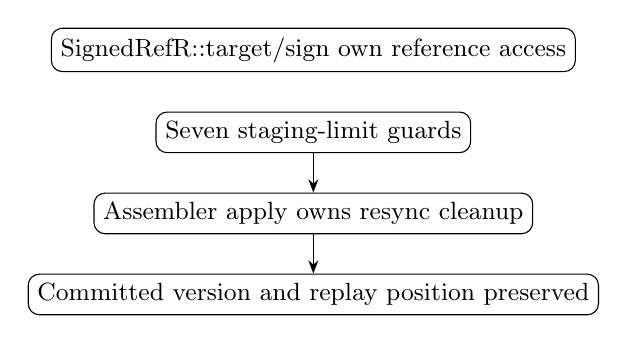
\begin{tikzpicture}[node distance=5mm, every node/.style={draw,rounded corners,font=\small},>=Stealth]
\node (refs) {SignedRefR::target/sign own reference access};
\node (limits) [below=of refs] {Seven staging-limit guards};
\node (error) [below=of limits] {Assembler apply owns resync cleanup};
\node (keep) [below=of error] {Committed version and replay position preserved};
\draw[->] (limits)--(error); \draw[->] (error)--(keep);
\end{tikzpicture}

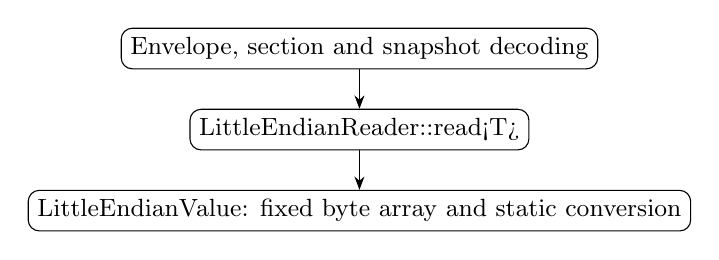
\begin{tikzpicture}[node distance=5mm, every node/.style={draw,rounded corners,font=\small},>=Stealth]
\node (clients) {Envelope, section and snapshot decoding};
\node (reader) [below=of clients] {LittleEndianReader::read<T>};
\node (value) [below=of reader] {LittleEndianValue: fixed byte array and static conversion};
\draw[->] (clients)--(reader); \draw[->] (reader)--(value);
\end{tikzpicture}

% 2026-10-12 evening: complete the remaining applicable catalogue work.
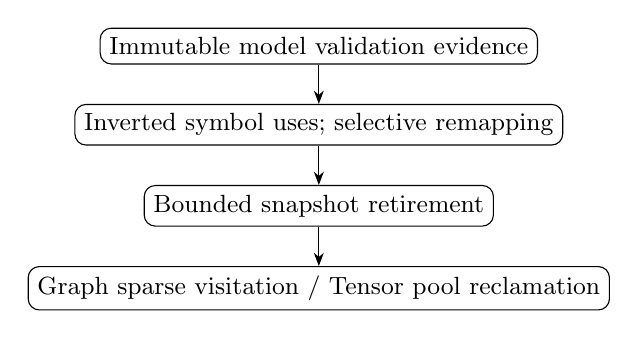
\begin{tikzpicture}[node distance=5mm, every node/.style={draw,rounded corners,font=\small},>=Stealth]
\node (proof) {Immutable model validation evidence};
\node (uses) [below=of proof] {Inverted symbol uses; selective remapping};
\node (retire) [below=of uses] {Bounded snapshot retirement};
\node (owners) [below=of retire] {Graph sparse visitation / Tensor pool reclamation};
\draw[->] (proof)--(uses); \draw[->] (uses)--(retire); \draw[->] (retire)--(owners);
\end{tikzpicture}

% 2026-10-12: caller-owned bounded scratch follows the committed algorithms.
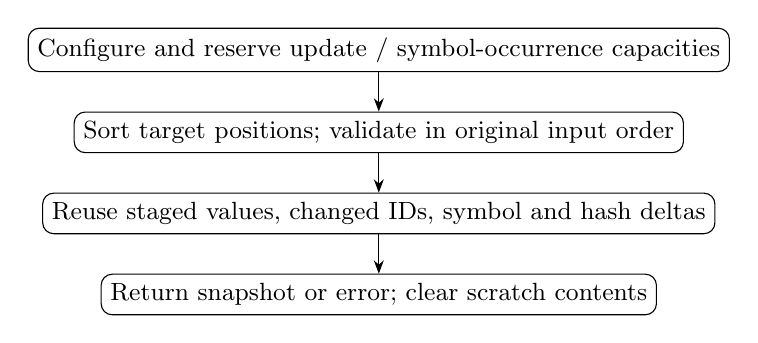
\begin{tikzpicture}[node distance=5mm, every node/.style={draw,rounded corners,font=\small},>=Stealth]
\node (reserve) {Configure and reserve update / symbol-occurrence capacities};
\node (order) [below=of reserve] {Sort target positions; validate in original input order};
\node (reuse) [below=of order] {Reuse staged values, changed IDs, symbol and hash deltas};
\node (clear) [below=of reuse] {Return snapshot or error; clear scratch contents};
\draw[->] (reserve)--(order); \draw[->] (order)--(reuse); \draw[->] (reuse)--(clear);
\end{tikzpicture}

% 2026-10-12: all catalogue candidates approved; first dependency pair.
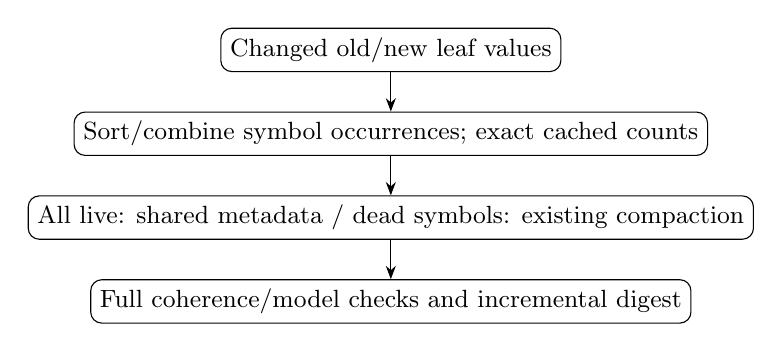
\begin{tikzpicture}[node distance=5mm, every node/.style={draw,rounded corners,font=\small},>=Stealth]
\node (values) {Changed old/new leaf values};
\node (delta) [below=of values] {Sort/combine symbol occurrences; exact cached counts};
\node (retain) [below=of delta] {All live: shared metadata / dead symbols: existing compaction};
\node (check) [below=of retain] {Full coherence/model checks and incremental digest};
\draw[->] (values)--(delta); \draw[->] (delta)--(retain); \draw[->] (retain)--(check);
\end{tikzpicture}

% 2026-10-12: private SkeletonForest child rows use stable count/prefix/scatter.
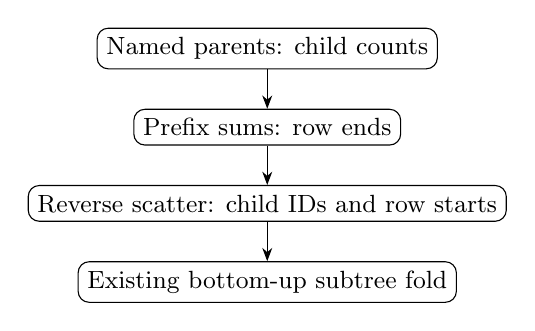
\begin{tikzpicture}[node distance=5mm, every node/.style={draw,rounded corners,font=\small},>=Stealth]
\node (count) {Named parents: child counts};
\node (prefix) [below=of count] {Prefix sums: row ends};
\node (scatter) [below=of prefix] {Reverse scatter: child IDs and row starts};
\node (fold) [below=of scatter] {Existing bottom-up subtree fold};
\draw[->] (count)--(prefix); \draw[->] (prefix)--(scatter); \draw[->] (scatter)--(fold);
\end{tikzpicture}

% PERF-1 2026-09-09T18:54:44+02:00: released course control -> measured optimization integration -> native/WASM parity -> GitHub/LAN publication.

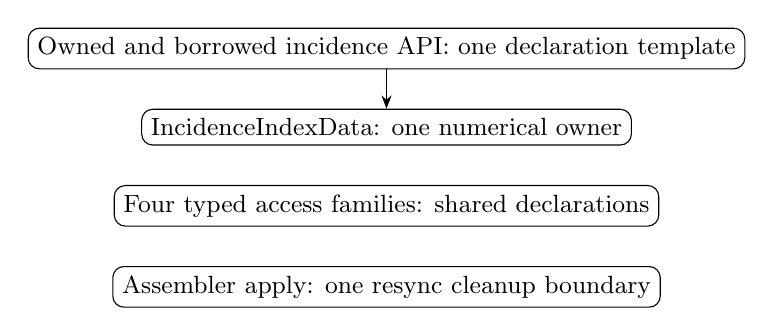
\begin{tikzpicture}[node distance=5mm, every node/.style={draw,rounded corners,font=\small},>=Stealth]
\node (api) {Owned and borrowed incidence API: one declaration template};
\node (data) [below=of api] {IncidenceIndexData: one numerical owner};
\node (access) [below=of data] {Four typed access families: shared declarations};
\node (apply) [below=of access] {Assembler apply: one resync cleanup boundary};
\draw[->] (api)--(data);
\end{tikzpicture}

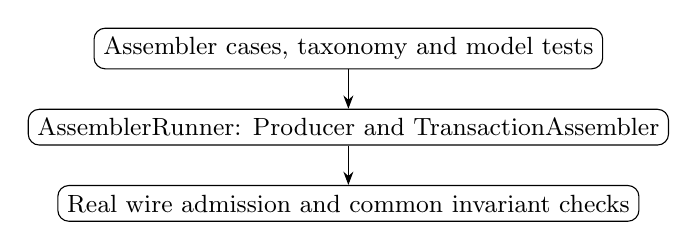
\begin{tikzpicture}[node distance=5mm, every node/.style={draw,rounded corners,font=\small},>=Stealth]
\node (tests) {Assembler cases, taxonomy and model tests};
\node (runner) [below=of tests] {AssemblerRunner: Producer and TransactionAssembler};
\node (wire) [below=of runner] {Real wire admission and common invariant checks};
\draw[->] (tests)--(runner); \draw[->] (runner)--(wire);
\end{tikzpicture}

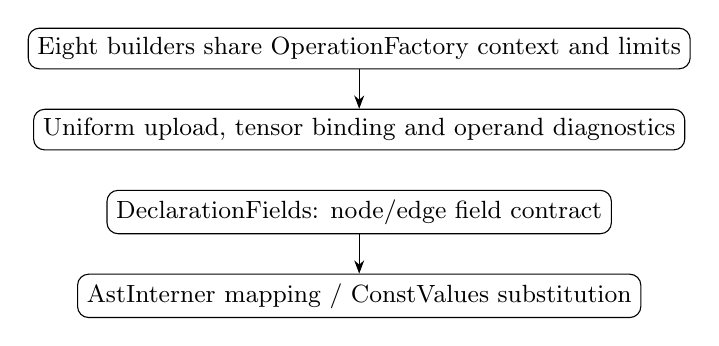
\begin{tikzpicture}[node distance=5mm, every node/.style={draw,rounded corners,font=\small},>=Stealth]
\node (gpu) {Eight builders share OperationFactory context and limits};
\node (upload) [below=of gpu] {Uniform upload, tensor binding and operand diagnostics};
\node (ast) [below=of upload] {DeclarationFields: node/edge field contract};
\node (passes) [below=of ast] {AstInterner mapping / ConstValues substitution};
\draw[->] (gpu)--(upload); \draw[->] (ast)--(passes);
\end{tikzpicture}

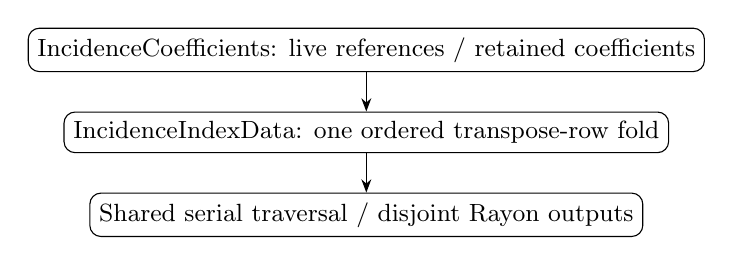
\begin{tikzpicture}[node distance=5mm, every node/.style={draw,rounded corners,font=\small},>=Stealth]
\node (coeff) {IncidenceCoefficients: live references / retained coefficients};
\node (row) [below=of coeff] {IncidenceIndexData: one ordered transpose-row fold};
\node (apply) [below=of row] {Shared serial traversal / disjoint Rayon outputs};
\draw[->] (coeff)--(row); \draw[->] (row)--(apply);
\end{tikzpicture}

% Tensor existing pool: budgeted epoch checks -> fairness and consumer gates

% Validation closure: short dispatch reproducer -> extracted binding checks -> oracle gates

% Test-only closure: same assertions in named helpers; all-target complexity gate

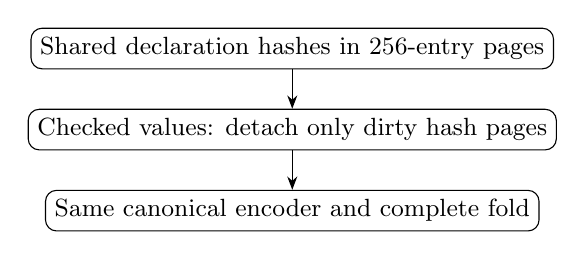
\begin{tikzpicture}[node distance=5mm, every node/.style={draw,rounded corners,font=\small},>=Stealth]
\node (basehash) {Shared declaration hashes in 256-entry pages};
\node (editpage) [below=of basehash] {Checked values: detach only dirty hash pages};
\node (foldhash) [below=of editpage] {Same canonical encoder and complete fold};
\draw[->] (basehash)--(editpage); \draw[->] (editpage)--(foldhash);
\end{tikzpicture}

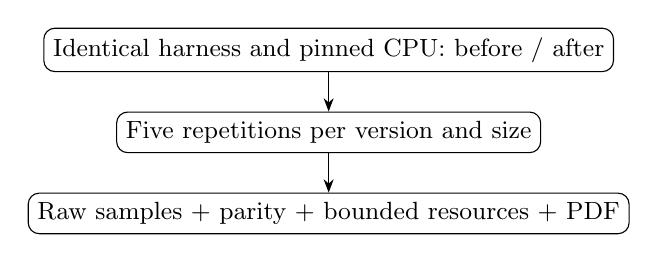
\begin{tikzpicture}[node distance=5mm,every node/.style={draw,rounded corners,font=\small},>=Stealth]
\node (matched) {Identical harness and pinned CPU: before / after};
\node (repeat) [below=of matched] {Five repetitions per version and size};
\node (evidence) [below=of repeat] {Raw samples + parity + bounded resources + PDF};
\draw[->] (matched)--(repeat);\draw[->] (repeat)--(evidence);
\end{tikzpicture}

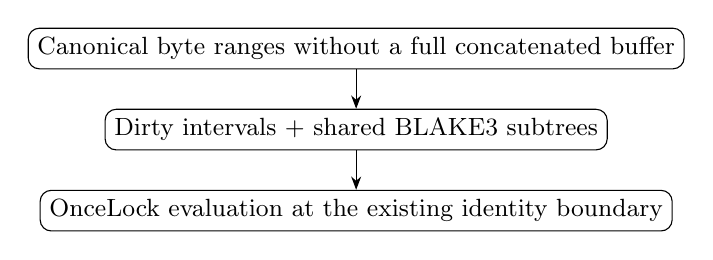
\begin{tikzpicture}[node distance=5mm,every node/.style={draw,rounded corners,font=\small},>=Stealth]
\node (virtual) {Canonical byte ranges without a full concatenated buffer};
\node (tree) [below=of virtual] {Dirty intervals + shared BLAKE3 subtrees};
\node (materialize) [below=of tree] {OnceLock evaluation at the existing identity boundary};
\draw[->] (virtual)--(tree);\draw[->] (tree)--(materialize);
\end{tikzpicture}

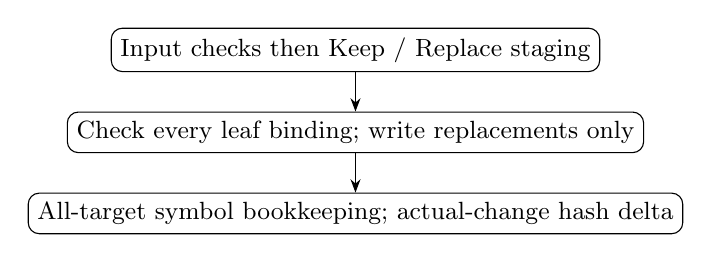
\begin{tikzpicture}[node distance=5mm,every node/.style={draw,rounded corners,font=\small},>=Stealth]
\node (checked) {Input checks then Keep / Replace staging};
\node (commit) [below=of checked] {Check every leaf binding; write replacements only};
\node (symbols) [below=of commit] {All-target symbol bookkeeping; actual-change hash delta};
\draw[->] (checked)--(commit);\draw[->] (commit)--(symbols);
\end{tikzpicture}

\par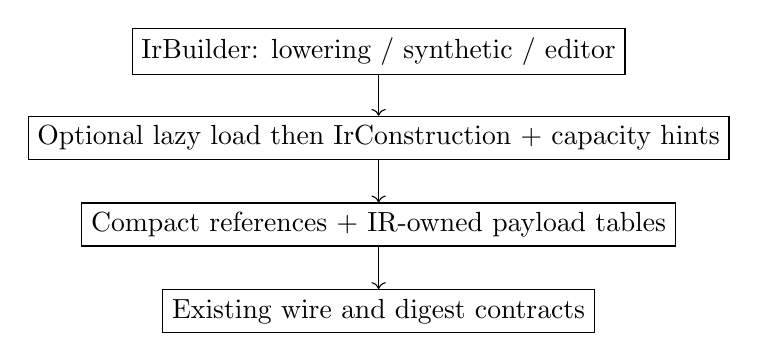
\begin{tikzpicture}[node distance=11mm,every node/.style={draw,align=center}]
\node(a){IrBuilder: lowering / synthetic / editor};\node(b)[below of=a]{Optional lazy load then IrConstruction + capacity hints};\node(c)[below of=b]{Compact references + IR-owned payload tables};\node(d)[below of=c]{Existing wire and digest contracts};\draw[->](a)--(b);\draw[->](b)--(c);\draw[->](c)--(d);\end{tikzpicture}

\par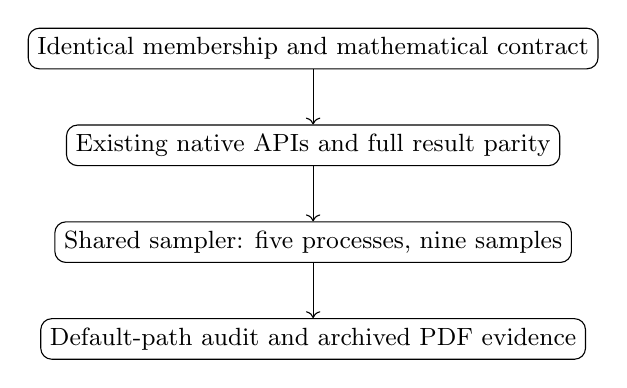
\begin{tikzpicture}[node distance=7mm,every node/.style={draw,rounded corners,align=center,font=\small}]
\node(a){Identical membership and mathematical contract};
\node(b)[below=of a]{Existing native APIs and full result parity};
\node(c)[below=of b]{Shared sampler: five processes, nine samples};
\node(d)[below=of c]{Default-path audit and archived PDF evidence};
\draw[->](a)--(b);\draw[->](b)--(c);\draw[->](c)--(d);\end{tikzpicture}

\par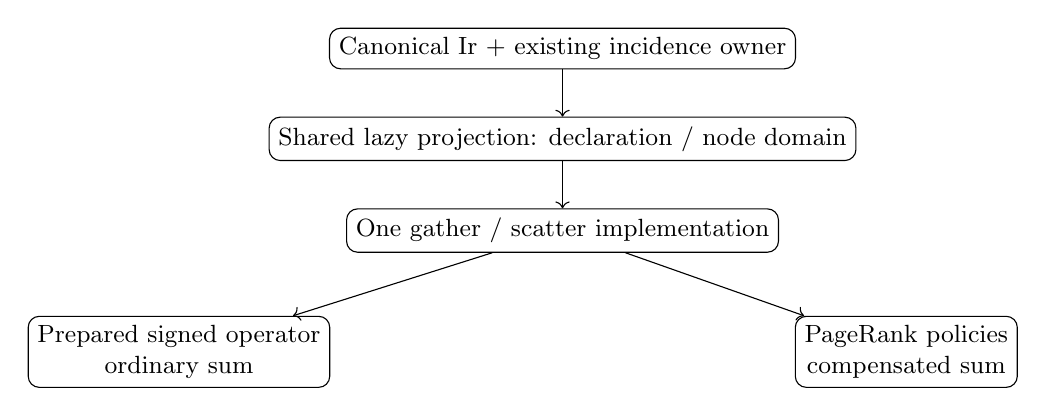
\begin{tikzpicture}[node distance=6mm,every node/.style={draw,rounded corners,align=center,font=\small}]
\node(a){Canonical Ir + existing incidence owner};
\node(b)[below=of a]{Shared lazy projection: declaration / node domain};
\node(c)[below=of b]{One gather / scatter implementation};
\node(d)[below left=8mm and 2mm of c]{Prepared signed operator\\ordinary sum};
\node(e)[below right=8mm and 2mm of c]{PageRank policies\\compensated sum};
\draw[->](a)--(b);\draw[->](b)--(c);\draw[->](c)--(d);\draw[->](c)--(e);\end{tikzpicture}

\par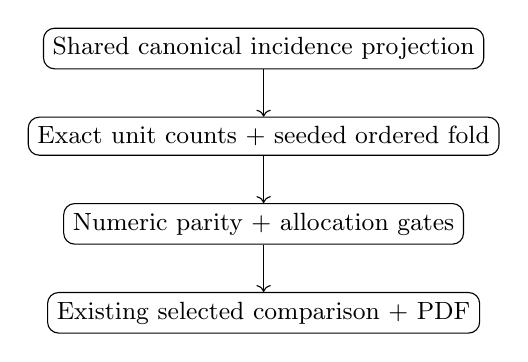
\begin{tikzpicture}[node distance=6mm,every node/.style={draw,rounded corners,align=center,font=\small}]
\node(a){Shared canonical incidence projection};
\node(b)[below=of a]{Exact unit counts + seeded ordered fold};
\node(c)[below=of b]{Numeric parity + allocation gates};
\node(d)[below=of c]{Existing selected comparison + PDF};
\draw[->](a)--(b);\draw[->](b)--(c);\draw[->](c)--(d);\end{tikzpicture}

\par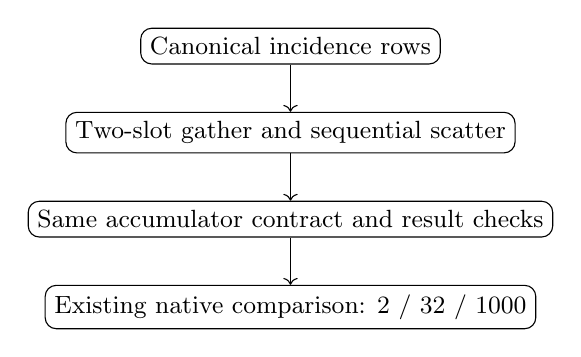
\begin{tikzpicture}[node distance=6mm,every node/.style={draw,rounded corners,align=center,font=\small}]
\node(a){Canonical incidence rows};
\node(b)[below=of a]{Two-slot gather and sequential scatter};
\node(c)[below=of b]{Same accumulator contract and result checks};
\node(d)[below=of c]{Existing native comparison: 2 / 32 / 1000};
\draw[->](a)--(b);\draw[->](b)--(c);\draw[->](c)--(d);\end{tikzpicture}

\par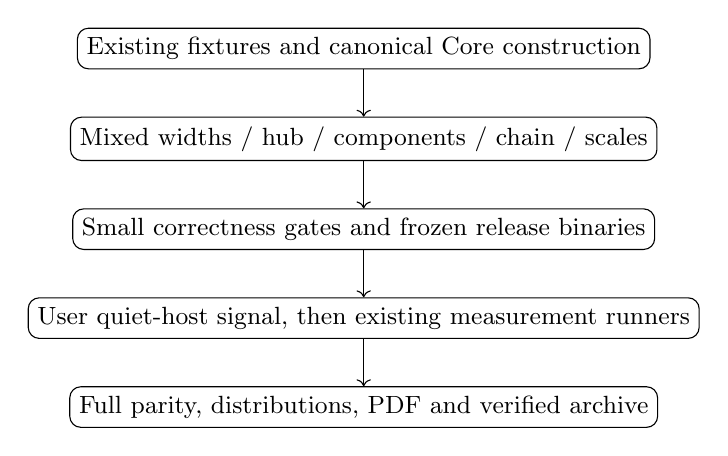
\begin{tikzpicture}[node distance=6mm,every node/.style={draw,rounded corners,align=center,font=\small}]
\node(a){Existing fixtures and canonical Core construction};
\node(b)[below=of a]{Mixed widths / hub / components / chain / scales};
\node(c)[below=of b]{Small correctness gates and frozen release binaries};
\node(d)[below=of c]{User quiet-host signal, then existing measurement runners};
\node(e)[below=of d]{Full parity, distributions, PDF and verified archive};
\draw[->](a)--(b);\draw[->](b)--(c);\draw[->](c)--(d);\draw[->](d)--(e);\end{tikzpicture}

% 2026-10-19: existing IR -> shared virtual incidence rows -> existing graph algorithms -> matched evidence

% 2026-10-19: Tensor numeric visitor -> Core IR projection -> Graph algorithms; entropy orders, bounds prune.

\par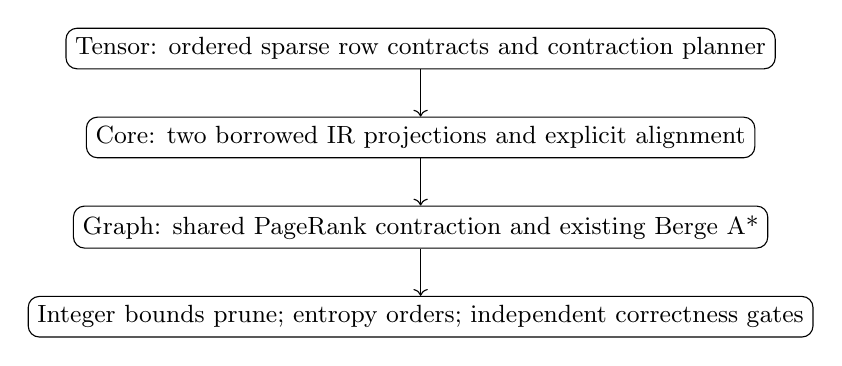
\begin{tikzpicture}[node distance=6mm,every node/.style={draw,rounded corners,align=center,font=\small}]
\node(a){Tensor: ordered sparse row contracts and contraction planner};
\node(b)[below=of a]{Core: two borrowed IR projections and explicit alignment};
\node(c)[below=of b]{Graph: shared PageRank contraction and existing Berge A*};
\node(d)[below=of c]{Integer bounds prune; entropy orders; independent correctness gates};
\draw[->](a)--(b);\draw[->](b)--(c);\draw[->](c)--(d);\end{tikzpicture}

\par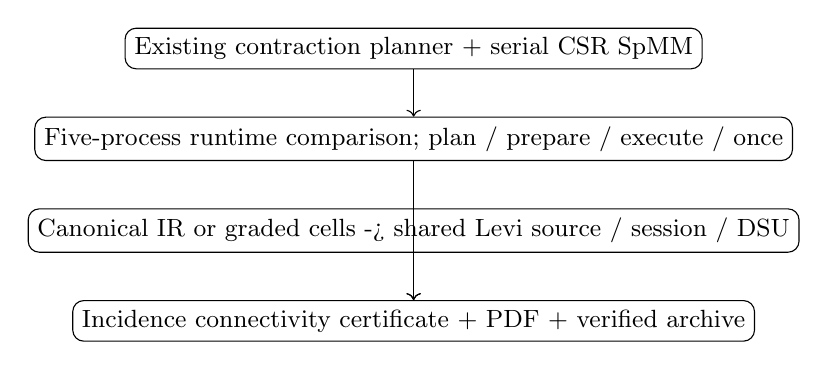
\begin{tikzpicture}[node distance=6mm,every node/.style={draw,rounded corners,align=center,font=\small}]
\node(a){Existing contraction planner + serial CSR SpMM};
\node(b)[below=of a]{Five-process runtime comparison; plan / prepare / execute / once};
\node(c)[below=of b]{Canonical IR or graded cells -> shared Levi source / session / DSU};
\node(d)[below=of c]{Incidence connectivity certificate + PDF + verified archive};
\draw[->](a)--(b);\draw[->](b)--(d);\draw[->](c)--(d);\end{tikzpicture}

\par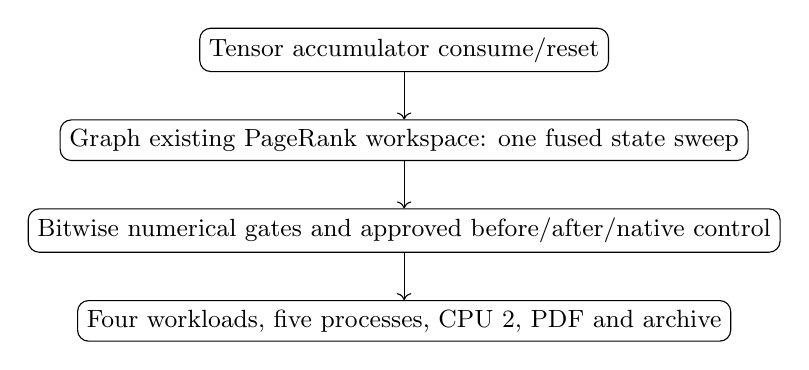
\begin{tikzpicture}[node distance=6mm,every node/.style={draw,rounded corners,align=center,font=\small}]
\node(a){Tensor accumulator consume/reset};
\node(b)[below=of a]{Graph existing PageRank workspace: one fused state sweep};
\node(c)[below=of b]{Bitwise numerical gates and approved before/after/native control};
\node(d)[below=of c]{Four workloads, five processes, CPU 2, PDF and archive};
\draw[->](a)--(b);\draw[->](b)--(c);\draw[->](c)--(d);\end{tikzpicture}

\par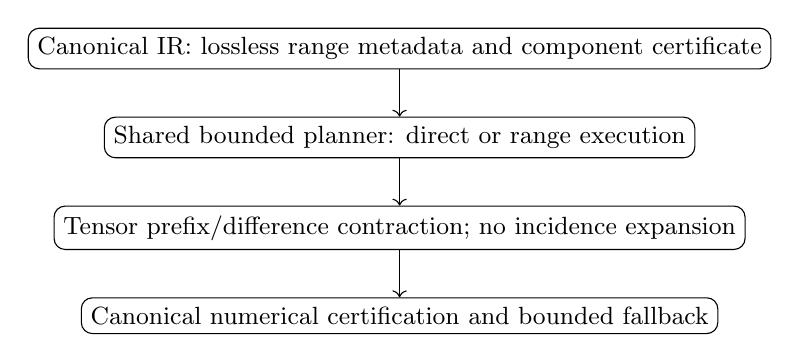
\begin{tikzpicture}[node distance=6mm,every node/.style={draw,rounded corners,align=center,font=\small}]
\node(a){Canonical IR: lossless range metadata and component certificate};
\node(b)[below=of a]{Shared bounded planner: direct or range execution};
\node(c)[below=of b]{Tensor prefix/difference contraction; no incidence expansion};
\node(d)[below=of c]{Canonical numerical certification and bounded fallback};
\draw[->](a)--(b);\draw[->](b)--(c);\draw[->](c)--(d);\end{tikzpicture}

\par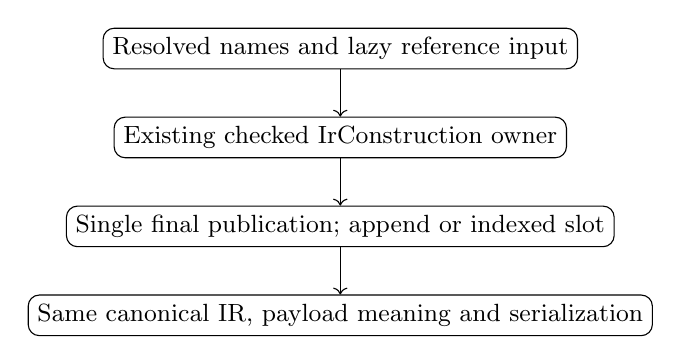
\begin{tikzpicture}[node distance=6mm,every node/.style={draw,rounded corners,align=center,font=\small}]
\node(a){Resolved names and lazy reference input};
\node(b)[below=of a]{Existing checked IrConstruction owner};
\node(c)[below=of b]{Single final publication; append or indexed slot};
\node(d)[below=of c]{Same canonical IR, payload meaning and serialization};
\draw[->](a)--(b);\draw[->](b)--(c);\draw[->](c)--(d);\end{tikzpicture}

\par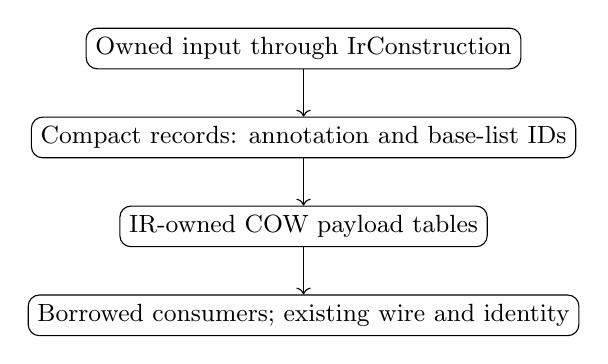
\begin{tikzpicture}[node distance=6mm,every node/.style={draw,rounded corners,align=center,font=\small}]
\node(a){Owned input through IrConstruction};
\node(b)[below=of a]{Compact records: annotation and base-list IDs};
\node(c)[below=of b]{IR-owned COW payload tables};
\node(d)[below=of c]{Borrowed consumers; existing wire and identity};
\draw[->](a)--(b);\draw[->](b)--(c);\draw[->](c)--(d);\end{tikzpicture}

\par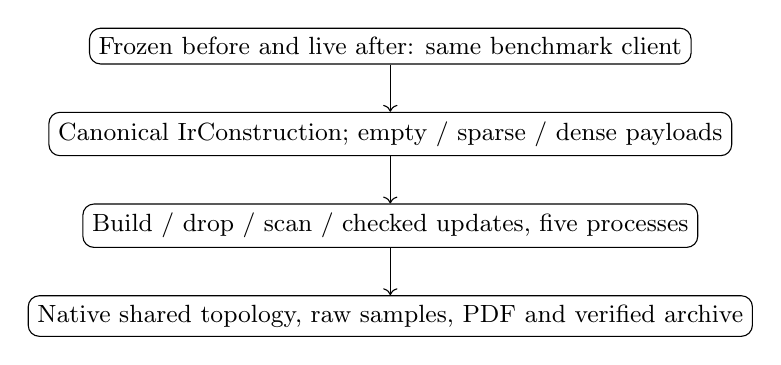
\begin{tikzpicture}[node distance=6mm,every node/.style={draw,rounded corners,align=center,font=\small}]
\node(a){Frozen before and live after: same benchmark client};
\node(b)[below=of a]{Canonical IrConstruction; empty / sparse / dense payloads};
\node(c)[below=of b]{Build / drop / scan / checked updates, five processes};
\node(d)[below=of c]{Native shared topology, raw samples, PDF and verified archive};
\draw[->](a)--(b);\draw[->](b)--(c);\draw[->](c)--(d);\end{tikzpicture}

\par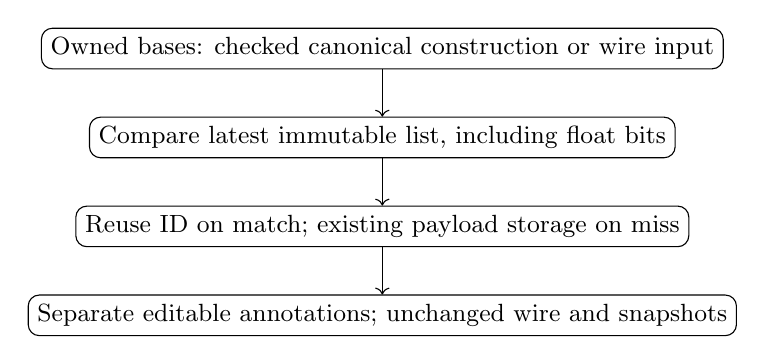
\begin{tikzpicture}[node distance=6mm,every node/.style={draw,rounded corners,align=center,font=\small}]
\node(a){Owned bases: checked canonical construction or wire input};
\node(b)[below=of a]{Compare latest immutable list, including float bits};
\node(c)[below=of b]{Reuse ID on match; existing payload storage on miss};
\node(d)[below=of c]{Separate editable annotations; unchanged wire and snapshots};
\draw[->](a)--(b);\draw[->](b)--(c);\draw[->](c)--(d);\end{tikzpicture}

\par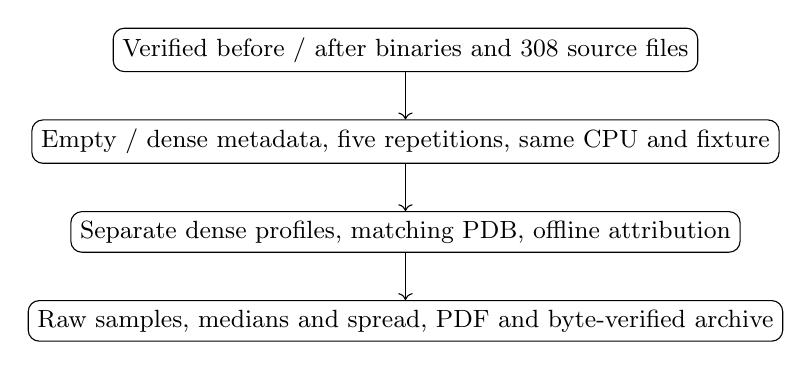
\begin{tikzpicture}[node distance=6mm,every node/.style={draw,rounded corners,align=center,font=\small}]
\node(a){Verified before / after binaries and 308 source files};
\node(b)[below=of a]{Empty / dense metadata, five repetitions, same CPU and fixture};
\node(c)[below=of b]{Separate dense profiles, matching PDB, offline attribution};
\node(d)[below=of c]{Raw samples, medians and spread, PDF and byte-verified archive};
\draw[->](a)--(b);\draw[->](b)--(c);\draw[->](c)--(d);\end{tikzpicture}

\par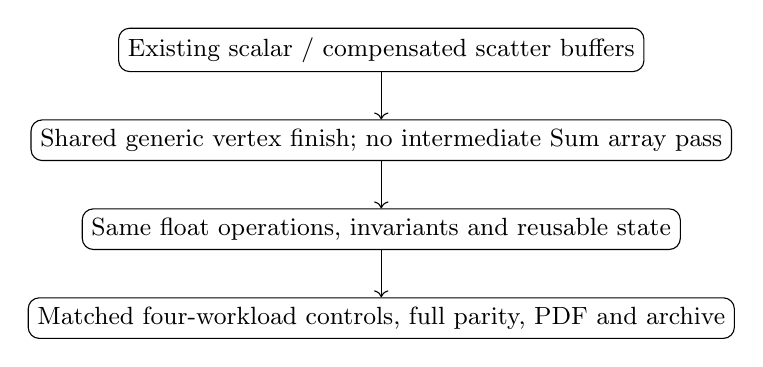
\begin{tikzpicture}[node distance=6mm,every node/.style={draw,rounded corners,align=center,font=\small}]
\node(a){Existing scalar / compensated scatter buffers};
\node(b)[below=of a]{Shared generic vertex finish; no intermediate Sum array pass};
\node(c)[below=of b]{Same float operations, invariants and reusable state};
\node(d)[below=of c]{Matched four-workload controls, full parity, PDF and archive};
\draw[->](a)--(b);\draw[->](b)--(c);\draw[->](c)--(d);\end{tikzpicture}

\par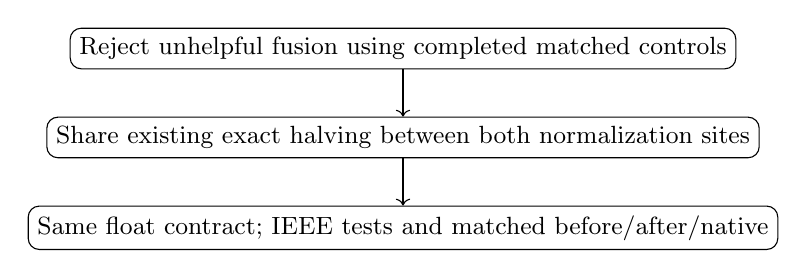
\begin{tikzpicture}[node distance=6mm,every node/.style={draw,rounded corners,align=center,font=\small}]
\node(a){Reject unhelpful fusion using completed matched controls};
\node(b)[below=of a]{Share existing exact halving between both normalization sites};
\node(c)[below=of b]{Same float contract; IEEE tests and matched before/after/native};
\draw[->](a)--(b);\draw[->](b)--(c);\end{tikzpicture}

\par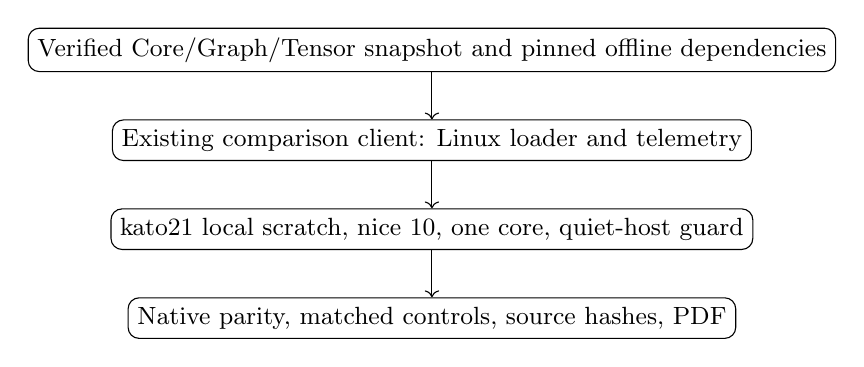
\begin{tikzpicture}[node distance=6mm,every node/.style={draw,rounded corners,align=center,font=\small}]
\node(a){Verified Core/Graph/Tensor snapshot and pinned offline dependencies};
\node(b)[below=of a]{Existing comparison client: Linux loader and telemetry};
\node(c)[below=of b]{kato21 local scratch, nice 10, one core, quiet-host guard};
\node(d)[below=of c]{Native parity, matched controls, source hashes, PDF};
\draw[->](a)--(b);\draw[->](b)--(c);\draw[->](c)--(d);\end{tikzpicture}

\par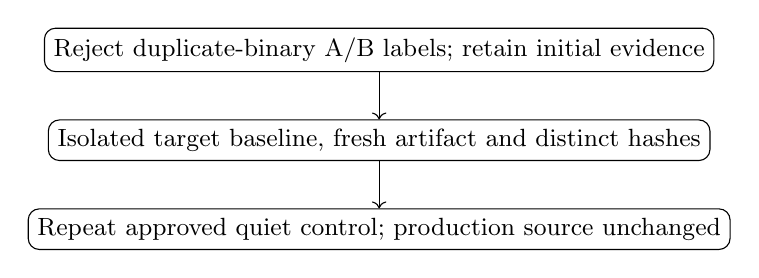
\begin{tikzpicture}[node distance=6mm,every node/.style={draw,rounded corners,align=center,font=\small}]
\node(a){Reject duplicate-binary A/B labels; retain initial evidence};
\node(b)[below=of a]{Isolated target baseline, fresh artifact and distinct hashes};
\node(c)[below=of b]{Repeat approved quiet control; production source unchanged};
\draw[->](a)--(b);\draw[->](b)--(c);\end{tikzpicture}

\par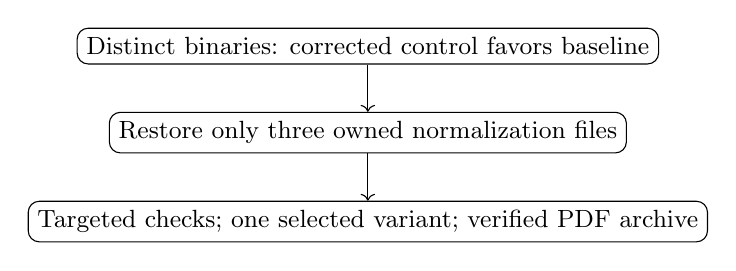
\begin{tikzpicture}[node distance=6mm,every node/.style={draw,rounded corners,align=center,font=\small}]
\node(a){Distinct binaries: corrected control favors baseline};
\node(b)[below=of a]{Restore only three owned normalization files};
\node(c)[below=of b]{Targeted checks; one selected variant; verified PDF archive};
\draw[->](a)--(b);\draw[->](b)--(c);\end{tikzpicture}

\par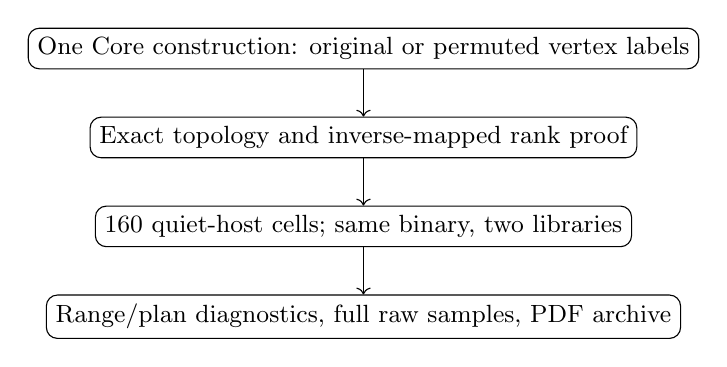
\begin{tikzpicture}[node distance=6mm,every node/.style={draw,rounded corners,align=center,font=\small}]
\node(a){One Core construction: original or permuted vertex labels};
\node(b)[below=of a]{Exact topology and inverse-mapped rank proof};
\node(c)[below=of b]{160 quiet-host cells; same binary, two libraries};
\node(d)[below=of c]{Range/plan diagnostics, full raw samples, PDF archive};
\draw[->](a)--(b);\draw[->](b)--(c);\draw[->](c)--(d);\end{tikzpicture}

\par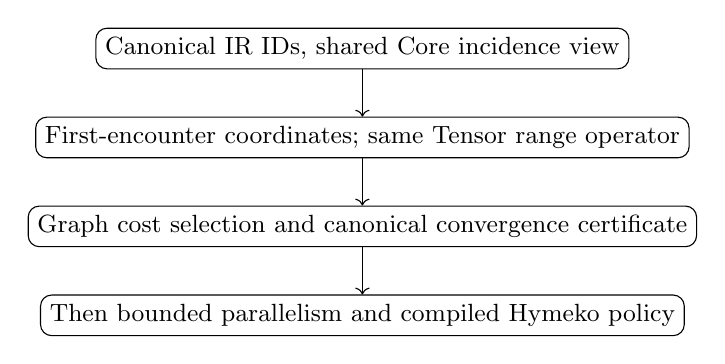
\begin{tikzpicture}[node distance=6mm,every node/.style={draw,rounded corners,align=center,font=\small}]
\node(a){Canonical IR IDs, shared Core incidence view};
\node(b)[below=of a]{First-encounter coordinates; same Tensor range operator};
\node(c)[below=of b]{Graph cost selection and canonical convergence certificate};
\node(d)[below=of c]{Then bounded parallelism and compiled Hymeko policy};
\draw[->](a)--(b);\draw[->](b)--(c);\draw[->](c)--(d);\end{tikzpicture}

\par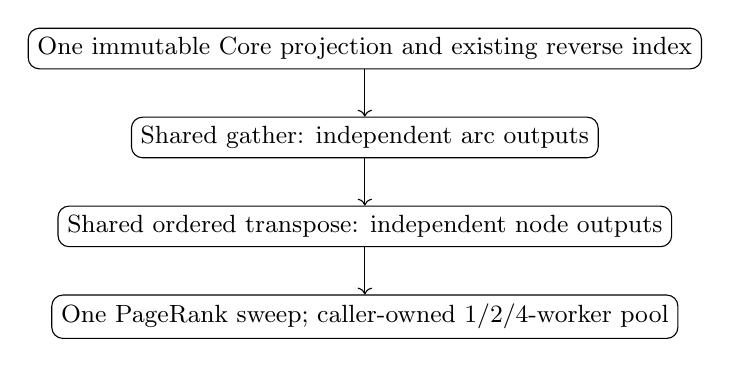
\begin{tikzpicture}[node distance=6mm,every node/.style={draw,rounded corners,align=center,font=\small}]
\node(a){One immutable Core projection and existing reverse index};
\node(b)[below=of a]{Shared gather: independent arc outputs};
\node(c)[below=of b]{Shared ordered transpose: independent node outputs};
\node(d)[below=of c]{One PageRank sweep; caller-owned 1/2/4-worker pool};
\draw[->](a)--(b);\draw[->](b)--(c);\draw[->](c)--(d);\end{tikzpicture}

\par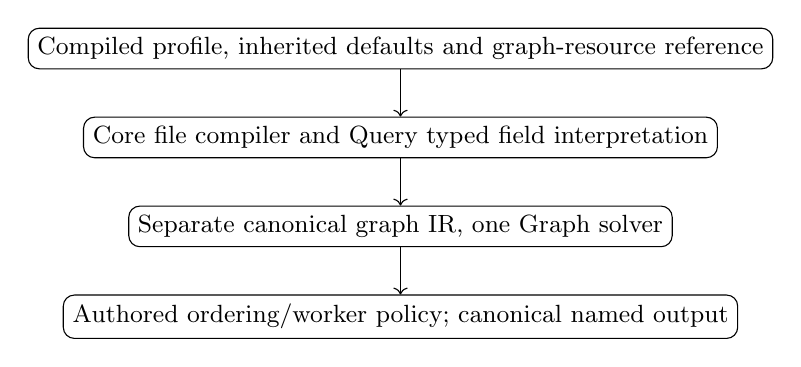
\begin{tikzpicture}[node distance=6mm,every node/.style={draw,rounded corners,align=center,font=\small}]
\node(a){Compiled profile, inherited defaults and graph-resource reference};
\node(b)[below=of a]{Core file compiler and Query typed field interpretation};
\node(c)[below=of b]{Separate canonical graph IR, one Graph solver};
\node(d)[below=of c]{Authored ordering/worker policy; canonical named output};
\draw[->](a)--(b);\draw[->](b)--(c);\draw[->](c)--(d);\end{tikzpicture}

\par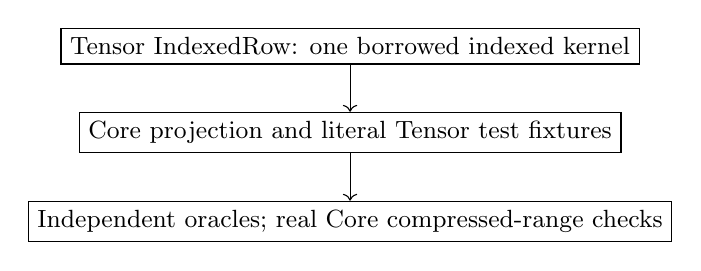
\begin{tikzpicture}[node distance=6mm,every node/.style={draw,align=center,font=\small}]
\node(a){Tensor IndexedRow: one borrowed indexed kernel};
\node(b)[below=of a]{Core projection and literal Tensor test fixtures};
\node(c)[below=of b]{Independent oracles; real Core compressed-range checks};
\draw[->](a)--(b);\draw[->](b)--(c);\end{tikzpicture}

\par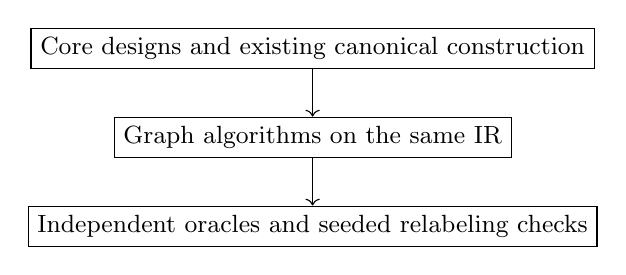
\begin{tikzpicture}[node distance=6mm,every node/.style={draw,align=center,font=\small}]
\node(a){Core designs and existing canonical construction};
\node(b)[below=of a]{Graph algorithms on the same IR};
\node(c)[below=of b]{Independent oracles and seeded relabeling checks};
\draw[->](a)--(b);\draw[->](b)--(c);\end{tikzpicture}

\par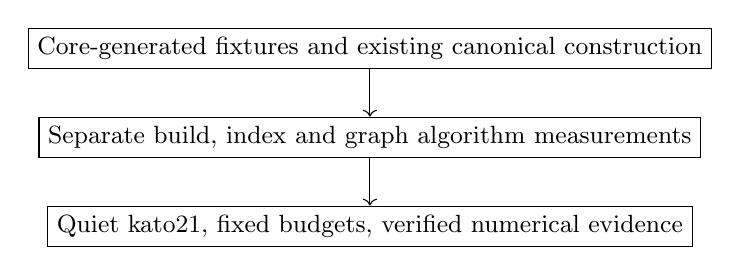
\begin{tikzpicture}[node distance=6mm,every node/.style={draw,align=center,font=\small}]
\node(a){Core-generated fixtures and existing canonical construction};
\node(b)[below=of a]{Separate build, index and graph algorithm measurements};
\node(c)[below=of b]{Quiet kato21, fixed budgets, verified numerical evidence};
\draw[->](a)--(b);\draw[->](b)--(c);\end{tikzpicture}
\end{center}

\section*{PERF-1 integration, 2026-09-09}
Created-at: 2026-09-09T18:54:44+02:00. ETA: approximately 60--90 minutes, based on cached builds,
existing 1-minute Core tests, 1--3 minute paired benchmark cells, SDK rebuild
and browser tests; no complete historical campaign rerun.
User approved saving the four-step strategy and executing step 1 in this turn.
Existing authorization: \texttt{APPROVED-CORE-EDIT: compiler-repeated-work};
the course-module-compilation approval was the user's affirmative reply to
that named scope, not a literal token. No new semantic or accelerator work.

Reuse the released course branches (Parser a528d98, Core 8623eb1) as bases.
The original dirty performance checkouts remain the preserved source of the
measured edits; independent integration worktrees hold the released control
and candidate during A/B builds. Core main's independent sparse commit is not
silently merged. Retire the temporary worktrees after evidence and publication.

Integrate only the existing grammar/string-scan optimizations, owned-record
benchmark adapter, root borrowing/shared canonical paths, compact Pruefer
state and single annotation-value resolution, plus their existing tests.
Keep final course tests and diagnostics from the published branches.
Affected additional paths: Parser grammar/lexer, existing benches/formats,
tests/format\_comparison.rs, scripts/format\_*.py and their tests, Parser
Cargo files and existing plan; Core canonical\_hash.rs, module\_store.rs,
resolve.rs, existing interning benchmark and frozen/ref/module-store tests,
Cargo pin/lock, generated SYMBOLS.md and docs/hymeko-platform-strategy.md;
SDK Cargo pin/lock, existing changelog/package README and generated package.
Root report exclusions remain. No Graph/Transformation/Tensor source change.

Use identical harnesses to build released control and integrated candidate.
Run large-case smoke before bounded measurements: 50k linked/long-text parser
and 50k mixed Core; 500k Core correctness/resource smoke where affordable.
Minimum five post-warmup samples, retain raw values, median/IQR/worst and peak
memory, binary/source/fixture hashes, affinity and environment. Reuse existing
Campaign/ProcessRunner, Criterion and plotting tools. A/A or repeated control
bounds ambient noise. More than ten percent stable regression requires
investigation; inconclusive is not pass. Existing profiles justify the
already-measured optimization mechanisms, not a fabricated combined speedup.
No tests/builds overlap timed cells. Max process peak 16 GiB, timed process
180 seconds. Preserve full-IR and corpus hashes, signed-reference diagnostics,
source provenance; run Parser, Core, native/Node/browser/Worker parity and
actual packed SDK installation. CPU tests only; no GPU performance claim.

Publication: provider before consumer, immutable Git revisions, one Core
identity, no local path patches shipped; verify GitHub and LAN refs. Reuse
current course branch without default-branch merge. Archive reports to Samba.
Rollback uses previous published SHAs and retained original SDK; never reset
or remove unrelated user work. PERF-2/3/4 remain planned at task completion.

\section*{Current full-IR characterization, 2026-09-13}
Created-at: 2026-09-13 15:37 +02:00. ETA: about 15 minutes for existing
target builds, correctness, bounded cells and report. User explicitly requests
the full IR benchmark and the compiled library size. No circular-buffer
remeasurement, profiler, production change or second compilation pipeline.
Reuse ModuleStore::compile through the existing interning benchmark: 50k numeric
and mixed sources, cold compile and cache hit reported separately. Reuse existing
canonical-CBOR corpus encode/decode cells as independent boundary measurements;
do not add phase medians to claim an end-to-end result. Ten or more post-warmup
Criterion samples, median/IQR/worst of per-sample iteration averages, no per-call
p99 claim. Run the exact public-facade corpus round-trip correctness test first.
Use existing measure\_peak\_memory.ps1 Program mode with explicitly built targets,
at most 16 GiB observed working set and 180 seconds per process. A single
same-scale smoke precedes repeated cells. Build/check work never overlaps timing.
Fresh release library build: default-empty features, no IPC/Arrow/GPU; report
rlib versus cdylib/PDB and inspect DLL exports. A small DLL without callable
Core exports is not the full linked Rust dependency footprint.
Affected tracked files: this existing plan.tex and rebuilt plan.pdf only.
Append results to reports/2026-09-07-compiler-repeated-work.md and reuse its
compiler-repeated-work evidence directory for raw samples, resource records and
plots. Preserve the other session's uncommitted circular-buffer bench, manifest
and plan changes. Rollback: revert this plan addendum; no runtime migration.

\section*{Post-extraction audit and performance, 2026-09-23}
Created-at: 2026-09-23 23:10 +02:00. ETA: 10--15 minutes including release
builds. User explicitly requested duplication inspection followed by performance
benchmarks. Reuse current dirty Core, Tensor and Nagare checkouts; no commits,
worktrees, source backups or production optimizations. Fetch succeeded in all
three. Pin the exact source hashes in the measurement record.

Audit the combined production sources of Core, WGPU, Tensor's numeric crate
and Nagare HNN with the existing token detector, using the same scope for Git
HEAD and current files. Report relocation separately from removed duplicates.
Inspect the surviving clone groups and distinguish shared contract duplication
from CPU/GPU strategies and different mathematical operators.

Artifact ledger: extend the existing interning benchmark with a semantic-digest
characterization group (full digest, cached read, checked leaf update including
clone/validation); reuse its deterministic source generator and public Core API.
Verify equality against the full digest before timing. Reuse the existing CSR
benchmark without copying its kernels or fixtures. Keep measurement opt-in.
Write reports/2026-09-23-core-tensor-audit-performance.md and raw JSON/logs/plots
under the existing reports/compiler-repeated-work directory, prefix cutover-.
No new runner or plan directory. Existing peak-memory runner and Criterion own
execution and sampling; no build/test overlaps measured cells.

Measure 50k-node cold/cached compilation and small/medium CSR SpMV/SpMM at
24 Rayon threads. Semantic digest uses a bounded 1000-node fixture with one
editable value. Minimum 10 warmed-up samples; median, inclusive IQR and worst
sample average (not per-call tail latency). Use historical same-host samples
only where source/config match; absence is a new baseline, not evidence of speedup.
Report OS, CPU, Rust version, flags, fixture digest and process peak working set.
Userspace RSS guard: 16 GiB; stop an individual timed process at 180 seconds.
A greater than 10 percent change is investigated before a causal claim. Retain
raw results even if the host is noisy. CPU results only; no GPU/remote claims.
Archive the report using the existing Samba synchronization tool. Rollback of
benchmark-only changes uses Git; generated measurement evidence stays in reports.

\section*{Canonical incidence owner, 2026-09-24}
Created-at: 2026-09-24 00:23 +02:00. ETA: 8--12 minutes for the focused
refactor, cached targeted tests and report. User explicitly requested a
struct/trait-oriented incidence API with hash() and bytes(); this authorizes
the Core canonical hashing edit. No benchmark or dependency change.

Extend canonical\_hash.rs with CanonicalIncidence, borrowing immutable IR,
and a private output trait implemented by Vec<u8> and the existing BLAKE3
hasher. One record iterator and encoder serve both methods. Normal hashing
streams ordered edges. Duplicate paths or wrapped u16 positions require
sorting lightweight records, using the same encoder without a byte arena or
fallback pipeline. Preserve the existing byte order, domains and hash config.
The existing public program-hash facade delegates to the owner; no old
incidence free functions or forwarding aliases remain.

Affected files: canonical\_hash.rs, existing frozen\_hash.rs tests, generated
SYMBOLS.md, this four-format plan and the existing Core/Tensor audit report.
Fresh fetch of all Core remotes succeeded; HEAD 10138bf equals the task
upstream and is three commits ahead of origin/main. Preserve all prior dirty
work; no new checkout, backup, commit or publication.

Verification: fixed payload bytes and header-plus-payload digest equality;
empty incidence, mixed signs, repeated targets, edge ordering, duplicate edge
paths, u16 arc/slot wrapping and long path truncation. Existing frozen whole
program vectors and generated forest/config corpus remain unchanged. Run only
the affected correctness target, library lint and touched-file format checks.
Worst input has many incidences with colliding paths: sorting holds record
descriptors, never duplicate encoded payloads. No speed or memory improvement
claim without measurement. Rollback is the scoped Git diff; no source backup.
Archive the amended report through the existing shared report-sync tool.
\section*{Pruefer owner, 2026-09-24}
Created-at: 2026-09-24 00:47 +02:00. ETA: 8--12 minutes for a focused
source refactor, cached correctness checks and report. The user explicitly
requests struct/trait orientation for Pruefer, authorizing the Core edit.
Core fetch succeeded on origin and github; task HEAD/upstream remains 10138bf,
three commits ahead of origin/main. Preserve existing uncommitted work.

Replace the tuple forest and free Pruefer orchestration with SkeletonForest
methods, a prepared CanonicalPrufer owner, and PruferTraversal implementing
Iterator. Store degree, neighbor XOR, live vertices and leaf heap in the
traversal. Share the existing CanonicalSink trait for byte/hash output; one
token iterator determines both. The canonical program hash uses this owner
directly. No compatibility wrappers or duplicate algorithm remain.
Preserve leaf priority (subtree hash, path tie, vertex), super-root handling,
iterative subtree folding, token order, headers and malformed-input behavior.

Affected files: canonical\_hash.rs, existing frozen\_hash.rs tests, generated
SYMBOLS.md, this four-format plan and the current Core/Tensor audit report.
Update stale helper-name comments in coherence.rs and the existing hierarchy
and test-oracle files; these edits do not change executable behavior.
Extend fixed hash vectors with public byte/hash parity, empty/single/multiple
roots, interleaved anonymous declarations and generated forest shapes/configs.
Exercise invalid cycle behavior explicitly. Run the frozen-hash and existing
ordinary hierarchy correctness cases, excluding the ignored resource probe;
library Clippy and touched-file formatting. No benchmark or dependency change.
Worst-case deep trees remain heap-traversed; hashing streams fixed-size tokens,
without constructing the full Pruefer payload. No measured speedup is claimed.
Rollback is the scoped Git diff, preserving the preceding incidence change.
No new checkout, source backup, commit or publication. Archive the final report.
\section*{Remaining canonical helpers, 2026-09-24}
Created-at: 2026-09-24 00:57 +02:00. ETA: 6--10 minutes for the Core boundary;
a public API migration may additionally require downstream checks. User requests
remaining free functions to move into their responsible structs.
Core fetched both remotes successfully; existing HEAD/upstream 10138bf remains.

CanonHashCfg owns domain-header initialization and chunk hashing. CanonicalPaths
owns construction from IR, reverse paths for resolution-boundary validation and
resolved strings. SkeletonForest owns its node-domain mapping. Reuse these
owners from Pruefer, incidence, path-index construction and program hashing;
remove their free helper bodies. No new struct solely to hold static utilities.
The user explicitly approved public entrypoint removal with consumer migration.
Promote CanonicalPaths::new/hash/validate; add DerivedPathIndex::new. Delete the
three free public entrypoints and migrate Core, web, XR, Kawamirai,
Transformation, Graph, the C++ Rust oracle and Nagare call sites. Keep manifest
and lockfile pins unchanged; local verification uses command-line path patches.
DerivedPathIndex is the existing owner for path-index construction.
The XR check also reaches the existing simulator-xr-publish checkout. Migrate
its callers and the primary simulator, Python binding and robot middleware
found by the workspace-wide search. Exclude inactive alternative checkouts and
the retired monorepo. Python's section-name adapter additionally requires the
already-existing CanonicalIrCbor enum case to compile against current Core.

Discovery ledger: find canonical\_hash.rs and existing consumer Rust files;
grep the three public names and all private helpers across framework/Nagare;
symbols confirm CanonHashCfg, CanonicalPaths, SkeletonForest and
DerivedPathIndex already own these concerns; read implementations and callers.
Verdict: EXTEND existing owners, remove free bodies, migrate callers in place.

Affected Core files: canonical\_hash.rs and focused frozen/path/namespace tests;
the existing plan bundle, symbol index and audit report. If public entrypoints
are migrated, their Core consumers and downstream callers are also in scope.
Keep canonical bytes, error variants and iteration behavior unchanged. Verify
fixed hash vectors, byte/hash parity, namespace failures, duplicate paths and
normal lookup behavior. No benchmark or dependency upgrade. Preserve prior edits;
rollback is only this continuation's diff. No new checkout or source backup.
\section*{Namespace validator owner, 2026-09-24}
Created-at: 2026-09-24 01:15 +02:00. ETA: 3--5 minutes. User requests a
dedicated validator struct. Core fetch succeeded on both remotes; task HEAD
10138bf equals upstream and remains three commits ahead of main. Preserve
the existing checkout and all preceding changes.

Discovery ledger: search IR/resolution for Validator and Validation owners
finds none; CanonicalPaths in SYMBOLS.md and its implementation own the present
validation. Read the method, namespace errors and all validation call sites.
Verdict: EXTEND canonical\_hash.rs with NamespaceValidator borrowing an existing
CanonicalPaths, and MOVE validation plus reverse-index preparation into it.
Remove CanonicalPaths::validate, with no forwarding method or free wrapper.
Keep namespace errors and canonical hash bytes unchanged. Migrate lowering,
CBOR validation and existing tests/bench call sites; retain shared path preparation.
Run namespace/frozen-vector and lowering-boundary correctness tests, CBOR tests,
compile the affected bench and run library lint. Update symbols and duplication
gate, append the existing report and archive. No measurements or dependency edits.
Rollback is the scoped diff; no backup or new checkout.
\section*{Subtree fold optimization, 2026-09-24}
Created-at: 2026-09-24 01:21 +02:00. ETA: 4--6 minutes. User requests a more
efficient subtree-hash implementation. Both Core remotes fetched; HEAD 10138bf
still equals task upstream. Preserve current checkout and prior edits.

Discovery: SkeletonForest::new is the sole owner of parent/children/root
construction; subtree\_hashes is its sole fold. Each named declaration is
inserted once under at most one valid named parent, or into roots. Therefore
a root-reachable cycle or shared child is impossible even for malformed input;
cycles and their descendants are disconnected from roots and retain zero hashes.
Verdict: EXTEND the existing method, no additional module or production owner.

Build one root-first order, fold it backwards, and write directly into a dense
zero-initialized HashId vector. Remove Enter/Exit frames, per-node Option state,
on-stack flags and final conversion. Reuse one child-hash scratch buffer sized
to maximum reachable fanout; skip it for leaves and single-child nodes. Use
in-place unstable lexicographic sort: equal hashes contain identical bytes, so
stability has no semantic effect. Cache the two configured named-leaf hashes
within the fold, never across calls or configurations. Preserve all hash bytes
and disconnected-component behavior. Complexity remains linear traversal plus
sum of child-sort costs; no measured speedup is claimed.

Verify existing frozen vectors/configuration corpus, dense-ID permutations,
deep/wide trees, mixed node/edge leaves, incidence multiplicity and malformed
cycles. Extend the existing cycle regression to include a rooted component and
a descendant of the disconnected cycle. Run only these correctness tests and
library Clippy; no benchmark or profile was explicitly requested. Update the
existing report, diagrams and symbol/duplication gates, then archive evidence.
Rollback is the scoped diff; no backup, new checkout or dependency change.
\section*{Current Core performance, 2026-09-24}
Created-at: 2026-09-24 01:30 +02:00. ETA: 3--5 minutes. The user explicitly
asks about performance benchmarks. Measure the existing interning Criterion
harness only: 50k canonical hash, cold/cached compile, and 1k full/cached digest
plus checked leaf update. Reuse the existing memory runner and raw-sample
summary machinery; no new benchmark implementation, source backup or worktree.
Both Core remotes fetched, HEAD 10138bf equals the task upstream.

Discovery/cached evidence: the September 23 report has paired compiler/digest
results. Its executable still exists and SHA256 matches 84f5f2261a8db3946b3d-
afa17fd789ba589c038006d40f0ce7ec1d16c5dee120. Run it twice before rebuilding,
then the current source twice, with explicit --bench, numeric 50k fixture,
24 Rayon threads, 1-second warmup and existing 10/20-sample groups. This compares
the accumulated canonical refactors, not the isolated last subtree change.
Verify source and canonical fixture hashes across binaries. Build time is excluded.

Budgets: each measured process below 16 GiB observed peak working set and
60 seconds wall time, expectation approximately 30 seconds from the prior
24.8-second five-cell run plus the hash cell. Preserve raw samples, report
median/IQR/worst sample average and two-run drift. Memory polling uses the
existing 100ms userspace cap; record its limits. Run sequentially without builds
or tests during timing. The Windows/275HX interactive host has background GUI
activity (largest observed process 0.156 CPU seconds per second); do not claim
a quiet-host release gate or attribute every difference to the subtree fold.
Investigate differences exceeding 10 percent within the measurement scope;
profiling remains unrequested, and causal speedup claims require separate evidence.
Keep source/manifest/executable provenance, amend this report and archive results.
No changes to production source, dependencies, public APIs or published pins.
\section*{Canonical hash batching, 2026-09-24}
Created-at: 2026-09-24 01:45 +02:00. ETA: 6--10 minutes including archive.
Continuation of the requested Core performance measurements and optimization.
Owner: Core canonical hash; the existing user authorization covers this private
implementation. Both remotes fetched; HEAD equals task upstream, three commits
ahead of main. Preserve unrelated dirty work and all public contracts.

Discovery ledger: CanonicalSink is the sole output strategy in canonical\_hash.rs;
no buffered hash sink exists in Core. Extend that strategy with one private
CanonicalHasher (configuration/header, fixed 16 KiB buffer, write, finish).
Replace the direct Hasher sink, not the encoder. Existing frozen\_hash tests,
interning\_bench, memory runner, report and plan bundle are reused. New measurement
artifacts belong to reports/compiler-repeated-work with batching prefixes.

Evidence: the existing resolved Pruefer profile includes 463 Hasher::update
samples, 255 ChunkState::update samples, and 371 path-string samples. These are
historical inclusive observations, not current causal attribution. Current
source issues per-field 1--32-byte updates. Test the bounded batching hypothesis
against the just-measured current binary (canonical hash 78.743 ms); do not claim
it explains the historical 6.6 percent regression without isolation.
Batch the 24-byte header in CanonHashCfg and pass the existing sorted child-hash
array as one contiguous slice. No alternate pipeline, dependencies or hash-version
change. Fixed buffer memory is O(1), independent of model size.

Acceptance: identical frozen hashes, configured headers, long UTF-8 prefixes,
wrapped incidence slots, empty streams, exact/full/partial buffer boundaries,
and repeated calls. Existing targeted correctness gate and library Clippy.
Two before and two after runs of only 50k canonical hash and cold compilation,
existing warmup/sample counts, sequentially, no concurrent build or test.
Expected 12--15 seconds per process, 40-second budget, 16 GiB observed peak cap.
Record executable hashes, raw medians/IQR/worst, peak working set and fixture
parity; interactive host remains a limitation. No fresh profiler run: reuse
existing attribution and measure the scoped change. Retain only if parity passes
and paired timings improve beyond ordinary run variation. Report and archive.
\section*{Remaining local duplication, 2026-09-24}
Created-at: 2026-09-24 01:58 +02:00. ETA: 4--6 minutes including archive.
User explicitly approved both identified cleanups and a fresh duplication audit.
Owner: Core. Existing task checkout fetched both remotes; no upstream drift.
Remove ir/common.rs and its module declaration; migrate the two integration-test
consumers to SignedRefR::target/sign. Search found no external use in the
framework/Nagare source trees. Public removal is intentional; no compatibility
facade, replacement module, dependency change or extra checkout.

Discovery: TransactionAssembler already owns abandon and the seven staging-limit
guards. Add one private staging\_limit\_exceeded method there; preserve guard
order, counter updates, all diagnostic strings, committed version and replay
position. Strengthen existing byte-limit, chunk-limit and superseded-drain tests
to verify cleanup and preserved committed/sequence state. Run the assembler unit
test module, the two migrated integration-test modules, library Clippy and fmt.
No benchmark or profiler is requested for this cleanup.

Compare the same token detector and scope before/after: entry 462 marked runs,
9588 marked lines, 185 scanned files. Separate source and test contributions;
inspect the remaining largest Core matches before calling any a duplicate
pipeline. Existing candidate inventory, report, symbol index and diagrams are
updated in place; report archived to the existing Samba destination.
\section*{Shared little-endian reader, 2026-09-24}
Created-at: 2026-09-24 02:12 +02:00. ETA: 5--7 minutes including archive.
User explicitly requests struct/trait/generic extraction of envelope readers.
Owner: Core ir\_stream. Both remotes fetched; existing task checkout is current.
Discovery found no shared endian reader in common or ir\_stream. New private
reader.rs owns LittleEndianReader over a borrowed byte slice and a
LittleEndianValue trait with associated fixed byte array. Generic read performs
one shared bounds-checked copy, then statically dispatches the type conversion.
A compact macro supplies primitive conversions for the four actual consumers:
u16, u32, u64, f32. SnapshotVersion implements the same private trait by reusing
its existing public conversion. No external reader API or dependency.

Migrate envelope fields, section-table fields, typed section-body copies and
snapshot counters. Remove the old rd functions and per-version closure.
Keep length/resource checks before reads/allocations, preserve exact validation
order and wire errors; a private reader called outside validated bounds may
panic, while public decoding must reject every truncated input. No pointer
casts, unsafe code, dynamic dispatch or parallel decoding implementation.

Tests: independent known bytes at unaligned offsets and exact buffer ends;
integer maxima, floating-point bit patterns, invalid offsets/short input; existing
envelope/section/version/codec unit tests and stream-admission integration tests.
Library Clippy, fmt, symbol-index and same-scope duplication checks. No performance
measurement requested. Update existing candidate inventory/report, archive evidence.
\section*{Incidence and access surfaces; assembler cleanup, 2026-09-24}
Created-at: 2026-09-24 02:39 +02:00. ETA: 6--8 minutes including archive.
Owner: Core. User approved incidence consolidation and further access/assembler
inspection. Both remotes fetched; existing task branch has no upstream drift.
Discovery finds one numeric incidence implementation already in IncidenceIndexData.
Share the 14 inherent delegating methods with a private declaration template,
parameterized by data lifetime: owned results borrow self, view results retain the
original data lifetime. Preserve Copy/two-pointer view layout, inherent call sites,
operator arithmetic/order and all public signatures. A trait-only replacement
would require consumer imports; a naive generic borrow shortens view lifetimes.
No new runtime abstraction, dependency, module or compatibility API.

In access.rs share the four typed iteration/count/containment declaration families.
Keep existing typed lookups and node/edge backlink checks, including the arc
exception. Templates describe a repeated public surface; they do not create a
second algorithm. Centralize transaction abandonment at public apply on every
ResyncRequired outcome; retain diagnostic state captured before cleanup and replay
bookkeeping rejection. Reset also reuses the existing abandon operation.

Extend existing incidence parity test with results surviving a short-lived view
(slice, iterator, data reference and operator plan). Existing assembler test driver
checks every resync preserves committed version/digest/sequence while clearing
staged/draining state. Run focused incidence/access integration tests and assembler
unit tests, library Clippy, formatting, symbol and duplication gates. No benchmark.
Compare the same detector against 461 marked runs / 9546 marked lines / 185 files;
separate declarations and test fixtures from actual pipeline duplication. Update
existing inventory and report; archive to Samba.
\section*{Assembler test runner, 2026-09-24}
Created-at: 2026-09-24 02:55 +02:00. ETA: 6--8 minutes: one test-only source
refactor, targeted test compilation and archive. User requests runner structs for
test duplication too. Owner: Core ir\_stream tests. Fresh fetch of both remotes;
upstream 0/0. Existing dirty checkout and all production behavior preserved.

Extend existing tests\_support with AssemblerRunner owning TransactionAssembler
and the existing Producer. Move the free apply helper and its real wire validation
and resync invariants into the runner. Reuse that path for step, expected outcome
and ordinary complete-transaction execution. Migrate unit tests, ignored taxonomy
probe and model tests; keep explicit bytes for exact/conflicting replay and expose
producer controls for sequence gaps, stream changes and exhaustion. No alternate
validator, test-only acceptance bypass, dependency or public production API.

Retain scenario-specific assertions and reference-model independence. Remove one
byte-identical duplicate replay test only after confirming the surviving test
covers all its assertions. Consolidate send/apply setup where bytes are used once;
keep fixtures reused by replay tests. Preserve raw message fields/order for every
migrated scenario. Existing correctness tests themselves prove runner behavior.

Affected: assembler.rs test modules, existing plan bundle, candidate inventory,
report and generated symbol index if needed. Source is CORE-protected; the user's
current runner request authorizes this test-only change. No production sections
will change. Run the assembler unit and model-test modules (taxonomy stays ignored),
Clippy for the library test target, rustfmt/diff checks, symbol and same-scope
duplication gates. No performance measurement. Before: 459 marked runs / 9279
marked lines, assembler 663 of which 607 in test code. A smaller source count must
not be bought by weakening tests or moving identical bodies into another file.
Worst cases retained: u64 sequence boundary, zero replay capacity, staged/drain
limits, randomized and exhaustive message streams. Restore only this task's patch
through Git if needed; no backup checkout. Append report and archive to Samba.
\section*{WGPU preparation and declaration traversal, 2026-09-24}
Created-at: 2026-09-24 03:08 +02:00. ETA: 10--15 minutes: eight backend builders,
two AST passes, focused correctness and archive. User explicitly approved WGPU
and traversal duplicate removal. Owner: Core checkout (hymeko\_wgpu backend and
hymeko\_core resolution). Fresh origin/github fetch; upstream 0/0; reuse checkout.
Existing roadmap invariants apply: canonical IR and numerical semantics unchanged.

WGPU: OperationFactory becomes the shared borrowed context for every builder,
with one OperationLimits value replacing eight per-operation limit structs.
Move typed uniform allocation/upload into that existing owner. GpuTensor owns
its binding-entry construction. A private OperandCheck owns the operand diagnostic
label and common required-value/shape-error construction. Remove six copies of
each helper and the rotor-local uniform builder. Preserve each prepare method's
validation order, diagnostics, kernel/layout binding positions, workgroup policy,
resource usage flags, typestate and operand lifetimes. No new preparation-time
collection, extra buffer, per-encode allocation, shader or numeric change.

AST: private DeclarationFields trait in existing sym\_ast.rs exposes borrowed
name/bases/optional children and mutable bases/children for NodeInner/EdgeInner.
An AstInterner struct owns the interner borrow; one generic declaration method
visits annotation/name/bases/body in existing order, with node/edge constructors
preserving None versus Some(empty). ConstValues owns one generic mutable
declaration walk. Arc ref-before-annotation substitution order remains explicit;
error short-circuiting and constant arithmetic stay unchanged. Remove replaced
free lowering/substitution helpers. Public entry points and parser dependency
remain stable; no parser checkout modification or new module.

Files: eight operations/*.rs builders, operations/mod.rs, resources.rs;
Core sym\_ast.rs, resolution/intern\_pass.rs and const\_resolve.rs; focused tests
in those owners as needed; existing plan/report/candidate/symbol artifacts.
These source paths are CORE-protected; the current user request authorizes them.
No dependency, branch, worktree, commit or publication change. Rollback only this
task's edits, preserving earlier dirty work.

Verification: Core intern/constant unit tests plus frozen identity/namespace
integration fixtures; strengthen order/optional-body/error precedence checks.
WGPU existing HSiKAN, entropy pooling, sparse scatter/highway/resident chain,
rotor attention/spike tests plus targeted SpMM/activation preparation and dispatch
cases. Inspect runners first; no profiling/benchmark opt-in. Execute GPU tests
serially and require actual adapter execution when available. Clippy for both
libraries, fmt/diff/symbol and duplicate gates. Before: 448 runs / 8996 marked
lines / 185 files. No performance claim; shared buffers retain existing allocation
sizes and ownership. Report actual results and any adapter skips; archive to Samba.

\section*{Incidence transpose row kernel, 2026-09-24}
Created-at: 2026-09-24 03:24 +02:00. ETA: 6--8 minutes, one production owner,
existing correctness fixtures, report and archive. User explicitly selected the
remaining index/prepared-plan calculation overlap. Core-protected source changes
are authorized by that request. Fresh origin/github fetch succeeded; upstream
0/0, existing dirty checkout retained. No dependency or public API change.

Introduce a private IncidenceCoefficients trait implemented by existing
IncidenceView and IncidenceOperatorPlan. The live strategy resolves the canonical
arc/ref coordinate; the prepared strategy reads its retained f64 coefficient.
IncidenceIndexData owns one ordered transpose-row fold, shared by direct serial,
prepared serial and Rayon applies. Share serial output traversal as well; preserve
its initial zeroing, partial-write behavior and untouched output tail. Rayon keeps
disjoint output partitioning and initial slice validation. Reuse the live coefficient
strategy during preparation. Preserve coefficient multiplication and summation
order, duplicate incidences, neutral references, signed zero and nonfinite policy.
The direct path propagates nonfinite values; preparation rejects the first offending
node in canonical node order. No dynamic dispatch, new retained array, per-apply
allocation, IR copy, matrix materialization, reordered arithmetic or automatic cache.
Bx and sparse topology construction remain in their existing owners.

Affected: incidence.rs, incidence\_precompute\_profile.rs correctness section,
existing plan bundle, candidate inventory, symbol index if changed and report.
Private trait and generic methods need no consumer migration. Restore only this
task's patch if necessary, retaining earlier uncommitted work; no backup checkout.

Tests: reuse index/view/prepared and independent oracle fixtures. Add a compact
runner covering cancellation-sensitive row order, duplicates, isolated nodes,
empty graph/arc, repeat apply, output tails, overflow/neutral nonfinite coefficients
and first-error node. Check bit parity including serial/Rayon; floating exceptional
results by classification where NaN payloads are unspecified. Inspect aggregate
selection first and keep ignored profiles disabled. Run incidence unit tests and
specific incidence correctness integration filters, Clippy, scoped fmt/diff,
symbol and duplication gates. Entry: 449 runs / 8543 marked lines / 185 files.
No performance experiment or speed claim: current request is consolidation.
Plan compile before source edit; write report and archive to Samba at completion.

\paragraph{Profiling continuation, 2026-10-11 17:11 +02:00.}
The user explicitly requests Core performance profiling and a fastest-framework
objective. Measure merged Core \texttt{b66cb4d} in the existing checkout; the source
tree is clean before this documentation amendment. ETA: 15--20 minutes for the
bounded initial characterization, including build, repeated cells, CPU capture and
analysis. Reuse \texttt{interning\_bench}, \texttt{ir\_bench},
\texttt{scripts/dev/measure\_peak\_memory.ps1}, \texttt{source\_manifest.ps1}
and \texttt{criterion\_report.ps1}. No new benchmark owner or dependency is needed.

\paragraph{Initial matrix and hypotheses.} First measure the existing 50k frontend
phases, full/cached semantic identity and a checked leaf update. Repeat the main
cells in two separate processes. After a bounded smoke, measure the existing
500k frontend's cold compile and structural hash, keeping its distinct source
identity. Cover true higher-arity structure with the existing IR hash cells
(1k and 10k nodes, arity 4 and 32). The competing explanations are parsing/lowering,
canonical encoding, and immutable-model copying/validation; attribute each using
symbolized stacks before selecting an optimization. Phase timings are not additive.

\paragraph{Measurement controls.} Criterion release with debug information, fixed
fixture hashes, raw samples, median/IQR/worst batch mean, and two repetitions.
Samply records separate 10-second CPU windows for cold compilation and semantic
digest/update paths; profiler times are not benchmark times. The existing Windows
monitor records peak working set and observes the 16 GiB cap. Keep individual
benchmark invocations below 180 seconds; log real progress, executable hashes,
commands, CPU/power context and host interference. OS profiler consent may require
user interaction; report it if capture is blocked. No services or other workloads
are stopped. Save a timestamped report and numerical/profile/plot artifacts under
\path{reports/2026-10-11-core-profile/}; archive with the shared report tool.

\paragraph{Acceptance and limits.} Existing Core correctness gates are green on
this revision (178 library, 152 IR verification and 7 doctests; Clippy clean).
Fixture parity assertions must pass in the benchmark too. This phase changes no
production code, hashes, public API or wire encoding. A profile justifies a
specific subsequent optimization; it does not establish a world ranking. Such a
ranking needs equivalent semantics, workloads and a separately agreed competitor
matrix. RL, renderer migration and unrelated numerical/GPU campaigns stay excluded.

\paragraph{Optimization continuation, 2026-10-11 18:13 +02:00.}
The user explicitly asks to proceed with optimization and to deliver PDF reports.
The completed CPU profile identifies symbol visitation and copying as update costs.
Core owns both changes: \path{module_store/execution/value_updates.rs} lazily copies
the base interner only when an update interns new text; \path{resolution/symbols.rs}
keeps its one typed walk but marks path/alias keys without rebuilding their hash maps.
Full hierarchy and model validation stay enabled. No representation, public API,
hash byte, error contract, snapshot isolation or symbol-lifetime change.

Extend the existing \path{benches/interning_bench.rs} with an explicit digest fixture
size and checked text updates. Preserve the original production binary/PDB pair after
building this same harness, then change production. Reuse the benchmark's existing
parity assertions; add a map-stability regression to symbol-compaction tests and run
it against the old implementation first. Existing mixed/nested-value, text lifetime,
invalid-input, old-reader and full/incremental parity tests remain discriminating gates.
Run the 1k and 50k update workloads in paired ABBA order, with raw samples and the same
Windows peak-working-set monitor. Measure full/cached digest controls at 1k. No new
benchmark owner or dependency. Preserve the 16 GiB / 180-second per-process budgets.

Expected implementation, tests and measurements: 20--30 minutes. The copy-elision
must retain the original symbol IDs until the existing compactor rewrites them;
text edits must still own their extended interner. Marking must validate every
symbol while leaving map keys and allocations intact; dense rewriting still rebuilds
maps. Reject a regression exceeding 10 percent and investigate its cause. Record the
result in a PDF beside the existing profiling artifacts, not a new Markdown report.
Rollback only the named optimization/test/benchmark hunks, preserving prior task work.
The existing checkout is reused on \texttt{perf/checked-value-update-symbols}; no new
worktree. No push or merge is performed without the requested notification.

\paragraph{Measured continuation, 2026-10-11 18:31 +02:00.}
The first ABBA sequence shows numeric-update gains but no consistent text-update
gain. The same symbol visitor allocates a worklist even for a numeric or DeclId
reference scalar, neither of which contains a SymId. Return immediately for these
two scalar roots; string/list traversal and all validation remain unchanged.
Preserve the first measured candidate and use separately named final ABBA samples,
against the same original binary and unchanged benchmark harness.

\paragraph{Second optimization, 2026-10-11 19:05 +02:00.}
The user authorizes the next measured Core optimization. The previous candidate's
symbolized update profile attributes 30.5 percent of selected stacks to hierarchy
coherence validation: copied path vectors, sorting and a second lookup table.
Core's existing \path{ir/coherence.rs} owns this validator; \path{PathKey} already
supports borrowed symbol-slice lookup. Borrow the existing paths and query the
existing Index instead of allocating per-path vectors and rebuilding a HashMap.
Keep deterministic declaration/path ordering with an unstable sort: Index keys are
unique, so ties cannot occur. All checks and report limits remain active.
Typed SymId paths also avoid the previous lossy u32 conversion; add a regression
for distinct 64-bit symbols with identical low 32 bits, plus exact ordered/capped
findings across reversed index insertion and nearest-prefix/empty-path cases.
This intentionally corrects false prefix matches for malformed wide symbol IDs;
ordinary graph findings, public API and hash/serialization algorithms are unchanged.

Extend the existing coherence integration suite. Reuse the preserved first-candidate
EXE/PDB as baseline and the unchanged interning benchmark. Run bounded 1k/50k smoke,
then numeric/text update ABBA comparisons and the 1k digest controls; 16 GiB cap,
under 180 seconds per process. Capture the optimized CPU profile and preserve source
manifests. Run Core library/unified-IR correctness, Clippy and downstream checks.
Report this second step and cumulative gains separately in PDF. Estimated duration:
15--25 minutes including build, paired measurements and reporting. Reuse this dirty
task checkout and branch; preserve prior changes. Rollback only this continuation's
coherence/test hunks. No commit, push or merge is requested by this continuation.

\end{document}
